% Resultados
\chapter{Resultados y validación} \label{ch:res}
  Este capítulo presenta los resultados obtenidos tras el desarrollo del proyecto y su comprobación mediante pruebas. Para ello, para cada escenario se va a comprobar que la infraestructura se despliega correctamente y posteriormente se va a validar que la conectividad entre los equipos es la esperada.

\section{Escenarios Smart Office}
  Se va a validar el despliegue de los escenarios Smart Office. Dado que la implementación es muy similar en ambos, se va a mostrar las pruebas realizadas sobre uno de ellos.

\subsection{Despliegue de la infraestructura}
 Lo primero es navegar hasta el directorio en el que se encuentran los ficheros \texttt{.tf}. Una vez ahí, es necesario ejecutar la orden \texttt{terraform init} para que se configure el provider correctamente, seguida de la orden \texttt{terraform apply} para que Terraform elabore un plan para alcanzar el estado deseado. Tras ejecutar \texttt{terraform apply}, Terraform mostrará una lista de los recursos a crear, modificar o eliminar para cumplir con el estado que marcan los ficheros de configuración. Tras la lista, aparecerá un prompt en el que sólo si escribimos \texttt{yes} Terraform procede a ejecutar las acciones necesarias para el despliegue.

  \begin{figure}[h]
  \centering
  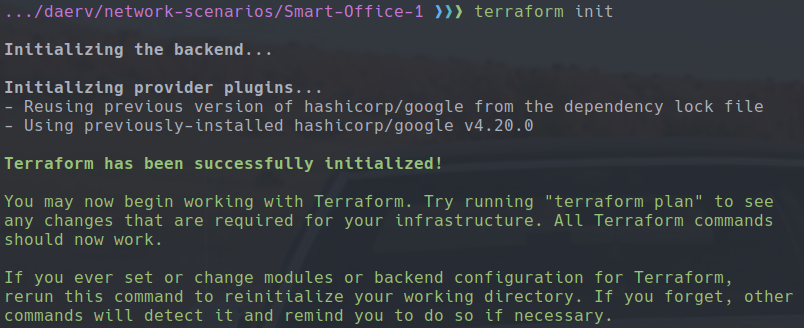
\includegraphics[width=0.8\textwidth]{../imgs/desarrollo/resultados/so/init.png}
  \caption{Ejecución del comando \texttt{terraform init}}
  \end{figure}
  
  \begin{figure}[h]
  \centering
  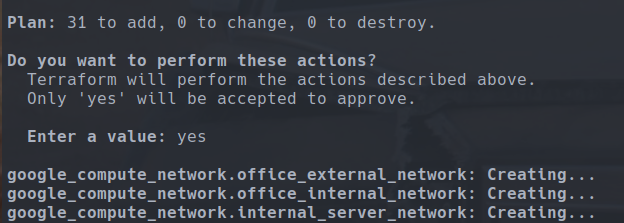
\includegraphics[width=0.8\textwidth]{../imgs/desarrollo/resultados/so/prompt.png}
  \caption{Prompt de confirmación tras la ejecución de \texttt{terraform apply}}
  \end{figure}

  Una vez se confirma la creación de los recursos, Terraform comienza a ejecutar el plan de creación de los recursos y va informando por la terminal sobre el estado de estos. Una vez se han creado todos, se nos informa y podemos ejecutar \texttt{terraform state list} para comprobar qué recursos hay desplegados: 

  \begin{figure}[h]
  \centering
  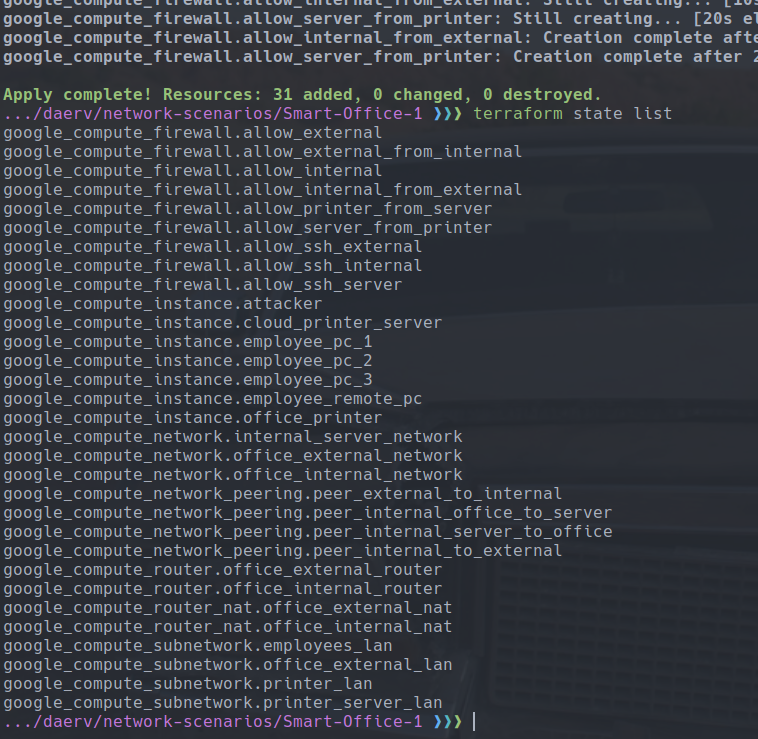
\includegraphics[width=0.75\textwidth]{../imgs/desarrollo/resultados/so/state.png}
  \caption{Ejecución del comando \texttt{terraform state list}}
  \end{figure}

  También podemos comprobar en GCP el despliegue de los diferentes elementos que componen el escenario accediendo a los distintos servicios, tal y como se muestra a continuación.

  \begin{figure}[h]
  \centering
  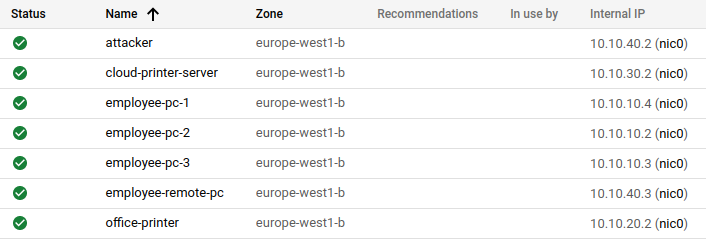
\includegraphics[width=\textwidth]{../imgs/desarrollo/resultados/so/instances.png}
  \caption{Instancias desplegadas en Google Compute Engine - Smart Office}
  \end{figure}

  \begin{figure}[h]
  \centering
  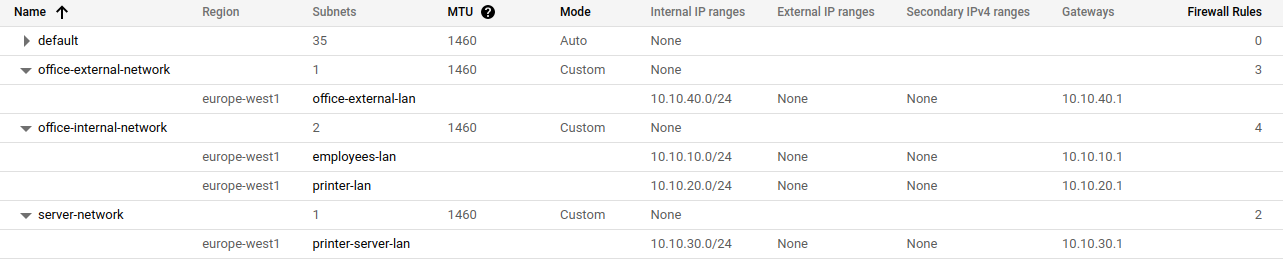
\includegraphics[width=\textwidth]{../imgs/desarrollo/resultados/so/vpcs.png}
  \caption{VPCs desplegadas - Smart Office}
  \end{figure}

  \begin{figure}[h]
  \centering
  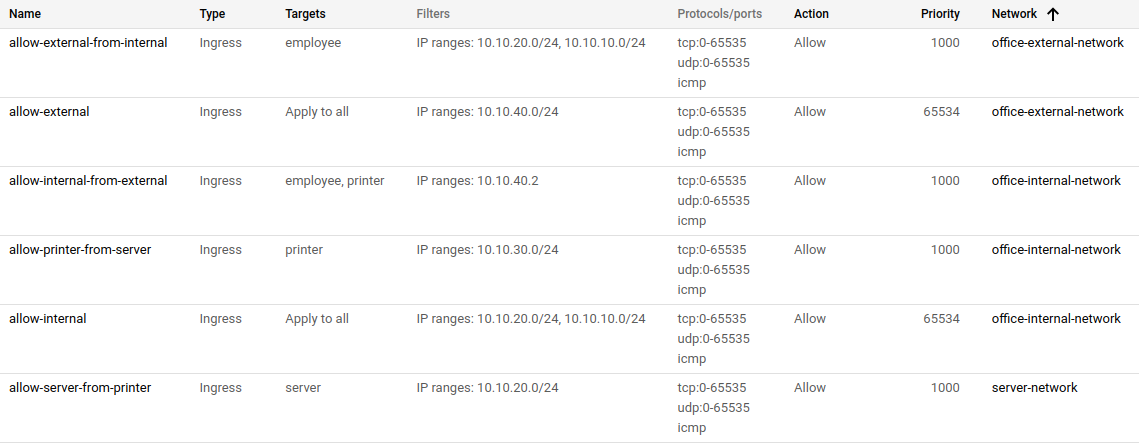
\includegraphics[width=\textwidth]{../imgs/desarrollo/resultados/so/fws.png}
  \caption{Reglas de FW aplicadas - Smart Office}
  \end{figure}
  \clearpage

\subsection{Tests}
  Para comprobar que la conectividad entre los elementos es la deseada según las reglas de firewall definidas en la tabla \ref{tab:fw1} se han creado una serie de tests de conectividad haciendo uso del servicio Network Intelligence de GCP:
  
  \begin{figure}[h]
  \centering
  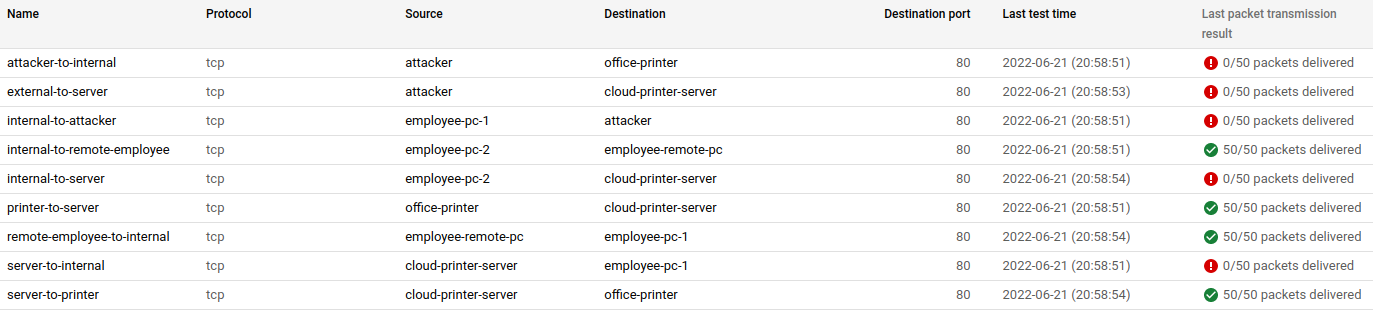
\includegraphics[width=\textwidth]{../imgs/desarrollo/resultados/so/tests.png}
  \caption{Tests de conectividad - Smart Office}
  \end{figure}

\section{Escenario Smart Home}
  Se van a presentar las mismas pruebas, esta vez para el escenario Smart Home. En este apartado, así como en el siguiente, se va a obviar la parte correspondiente a los comandos de Terraform para evitar redundancia. 

\subsection{Despliegue de la infraestructura}
  Se muestra a continuación como la infrestructura se ha creado correctamente en GCP:

  \begin{figure}[h]
  \centering
  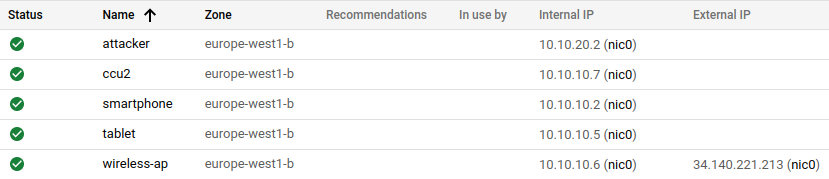
\includegraphics[width=\textwidth]{../imgs/desarrollo/resultados/sh/instances.png}
  \caption{Instancias desplegadas en Google Compute Engine - Smart Home}
  \end{figure}

  \begin{figure}[h]
  \centering
  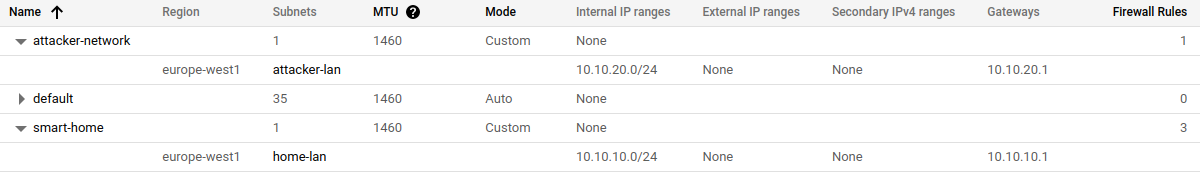
\includegraphics[width=\textwidth]{../imgs/desarrollo/resultados/sh/vpcs.png}
  \caption{VPCs desplegadas - Smart Home}
  \end{figure}
  \clearpage

  \begin{figure}[h]
  \centering
  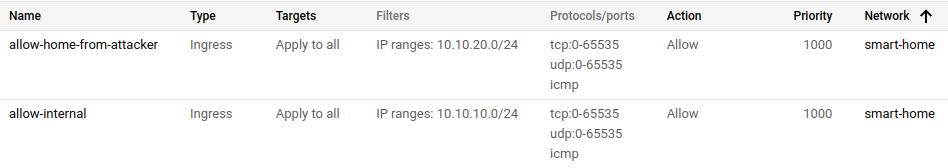
\includegraphics[width=\textwidth]{../imgs/desarrollo/resultados/sh/fws.png}
  \caption{Reglas de FW aplicadas - Smart Home}
  \end{figure}

\subsection{Tests}
  En este escenario se han definido los siguientes tests:

  \begin{figure}[h]
  \centering
  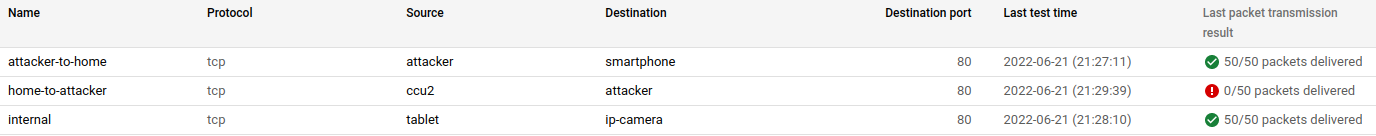
\includegraphics[width=\textwidth]{../imgs/desarrollo/resultados/sh/tests.png}
  \caption{Tests de conectividad - Smart Home}
  \end{figure}

  Adicionalmente, accedemos a una de las instancias de la red local de la casa a través de SSH (es necesario crear una regla de FW que lo permita) y vemos que tiene acceso a Internet a través de la IP pública de la instancia wireless-ap y que cuenta con Docker instalado, lo que verifica el funcionamiento de los scripts \texttt{proxy-config.tftpl} y \texttt{docker-proxy-provisioning.tftpl} pasados como parámetro:

  \begin{figure}[h]
  \centering
  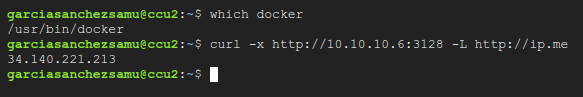
\includegraphics[width=\textwidth]{../imgs/desarrollo/resultados/sh/tests2.png}
  \caption{Tests de aprovisionamiento - Smart Home}
  \end{figure}
  \clearpage

\section{Escenario SCADA}
  Al igual que los apartados anteriores, se va a presentar el despliegue y los tests correspondientes al escenario SCADA.
  
\subsection{Despliegue de la infraestructura}
  A continuación se muestra, al igual que para el resto de escenarios, imágenes que verifican el despliegue de la infraestructura en Google Cloud. 

  \begin{figure}[h]
  \centering
  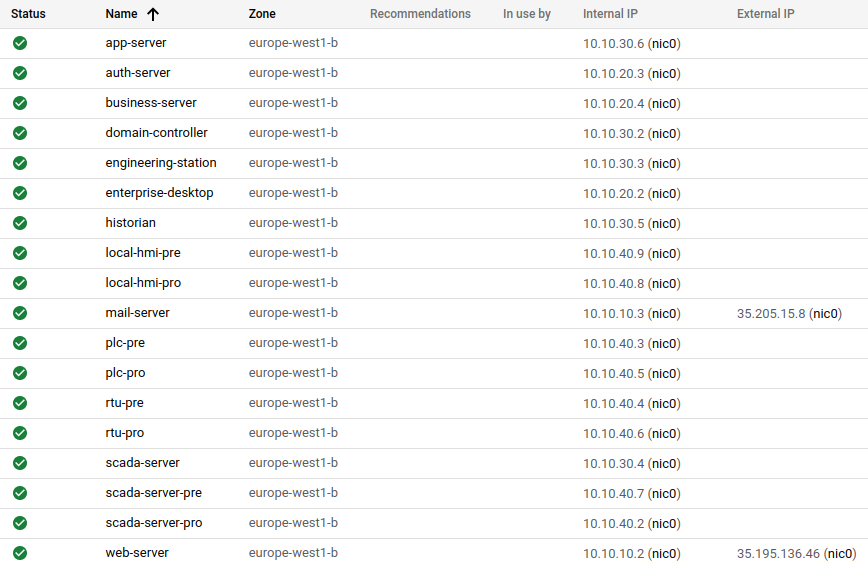
\includegraphics[width=\textwidth]{../imgs/desarrollo/resultados/scada/instances.png}
  \caption{Instancias desplegadas en Google Compute Engine - SCADA}
  \end{figure}

  \hfill{5cm}

  \begin{figure}[h]
  \centering
  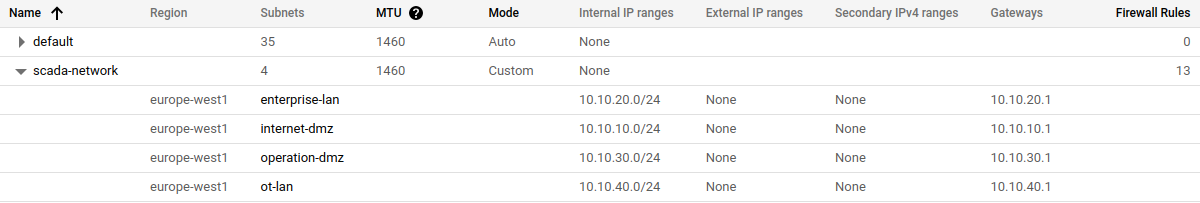
\includegraphics[width=\textwidth]{../imgs/desarrollo/resultados/scada/vpcs.png}
  \caption{VPCs desplegadas - SCADA}
  \end{figure}
  \clearpage

  \begin{figure}[t]
  \centering
  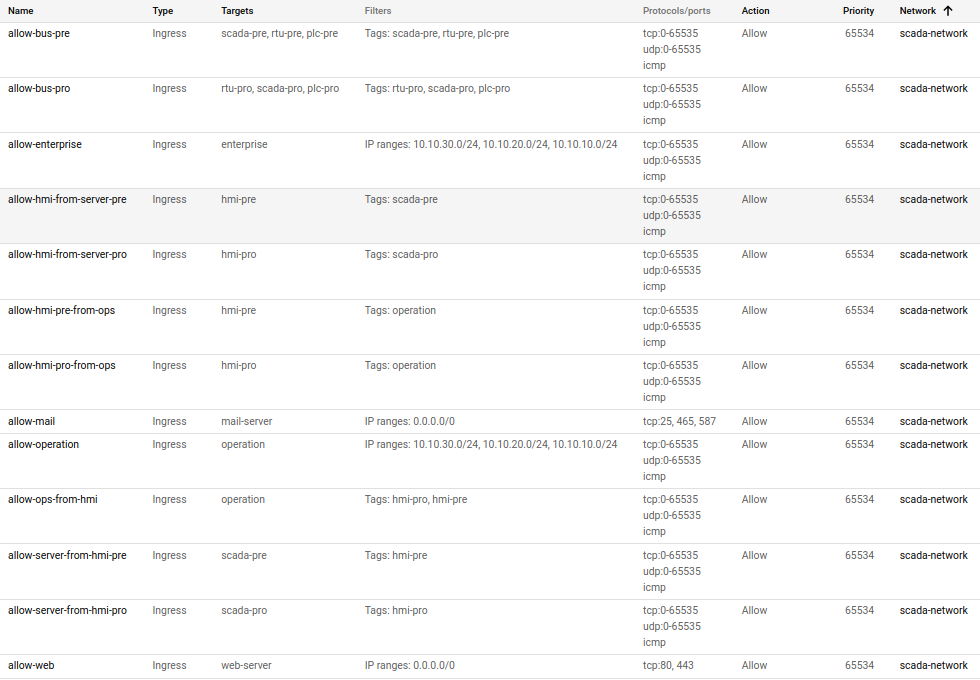
\includegraphics[width=\textwidth]{../imgs/desarrollo/resultados/scada/fws.png}
  \caption{Reglas de FW aplicadas - SCADA}
  \end{figure}
  
\subsection{Tests}
  Los siguientes tests de conectividad han sido definidos:

  \begin{figure}[h]
  \centering
  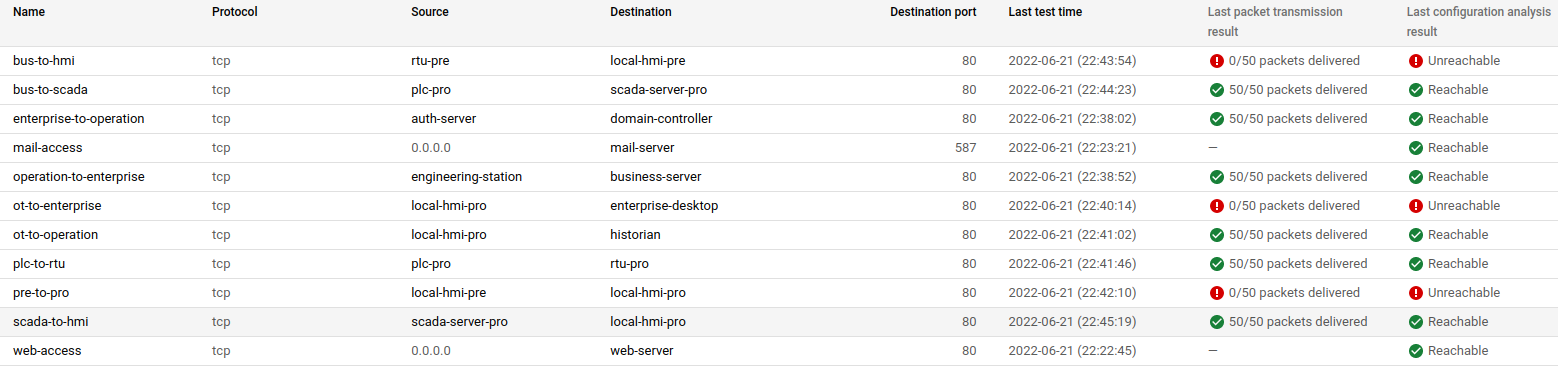
\includegraphics[width=\textwidth]{../imgs/desarrollo/resultados/scada/tests.png}
  \caption{Test de conectividad - SCADA}
  \end{figure}
  \clearpage

  Por último se verifica el funcionamiento del script \texttt{docker-provisioning.tftpl}. Para ello accedemos a la IP pública del servidor web desde el ordenador host y comprobamos que está ejecutando el software \textit{nginx} en el puerto 80.

  \begin{figure}[h]
  \centering
  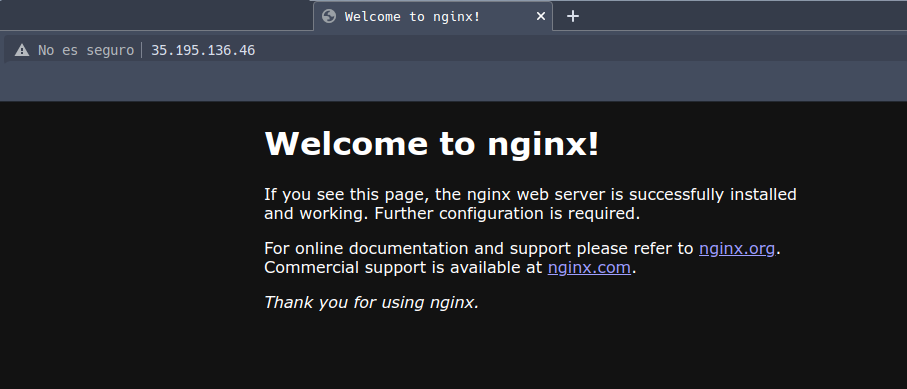
\includegraphics[width=\textwidth]{../imgs/desarrollo/resultados/scada/nginx.png}
  \caption{Test de aprovisionamiento - SCADA}
  \end{figure}
